\section{Advanced Connectivity Options}
\subsection{Setting a static IP Through Config}
Once you've successfully SSH's into your Pi, it's a good idea to configure the networking options in the config files directly.

Use a text editor such as nano to open /etc/dhcpcd.conf as sudo user, and edit it to the following:
\begin{lstlisting}
# Static IP profile for eth0
profile static_eth0
static ip_address=192.168.137.15/24
static routers=192.168.137.1
static domain_name_servers=192.168.137.1 8.8.8.8

# Ethernet interface configuration 
interface eth0
fallback static_eth0

# Wireless configuration
interface wlan0
metric 200
\end{lstlisting}

\subsection{Providing your Pi with wireless Internet Access}
There are two possible methods of this that will be presented, each with it's own advantages and disadvantages.

The first is using Ethernet passthrough from your computer to the Raspberry Pi. This leaves the WiFi free to host your own access point, and you can host services such as a Node-Red server or media center on the Pi.

The second involves connecting to a wireless network. In the example we give you, we're only going to add a connection to Eduroam. While you could host other services on the Pi when using WiFi connectivity, it would require some access to port forwarding and other things that ICTS unfortunately won't allow.

It is recommended that you use Ethernet pass through for the practicals.

\subsubsection{Using WiFi to Ethernet passthrough to give your Pi internet access}
There may be a situation in which you want your Pi to work as an access point rather than using the WiFi interface to provide the Pi with internet access. In this situation, you need to get internet access through the ethernet port. If you're connected to Windows, you can use network sharing. Complete the following to enable network sharing:

\textbf{Windows}\\
\begin{enumerate}
    \item Ensure the Pi is unplugged
    \item Right click on your network option in Windows taskbar
    \item Select  "Open Network \& Internet Settings", on the lower right hand side of the screen.
    \item Select "Change Adapted Options"
    \item Right click on your WiFi network and select "Properties"
    \item Click the "Sharing" tab, and enable the first checkbox \footnote{This setting is what forces us to have to use the subnet 192.168.137.x.}
    \item Select the Ethernet connection that your Pi will be using in the drop down box (Usually just "Ethernet", but may be different if there are multiple Ethernet posts on your system)
\end{enumerate}

\begin{figure}[H]
\centering
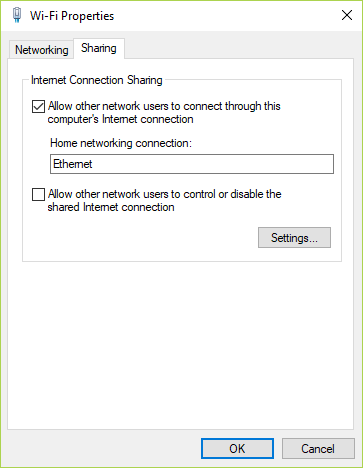
\includegraphics[width=0.5\columnwidth]{Figures/windowspassthrough}
\caption{Using WiFi to Ethernet passthrough in Windows}
\label{fig:windowspassthrough}
\end{figure}

\textbf{Ubuntu}\\
\begin{enumerate}
    \item Ensure the Pi is unplugged and turned off.
    \item Open a terminal and run \verb|nm-connection-editor|
    \item Select the wired connection you'd like to share your WiFi to
    \item Select the IPv4 settings tab
    \item Under Method, select "Shared to other computers"
    \item under the IP addresses, click "Add" and enter in an address of 192.168.137.1, and a netmask of 24
    \item Select "Save", and close the windows
    \item Plug in the Pi, start an SSH session and see if you can ping google.co.za
\end{enumerate}

\begin{figure}[H]
\centering
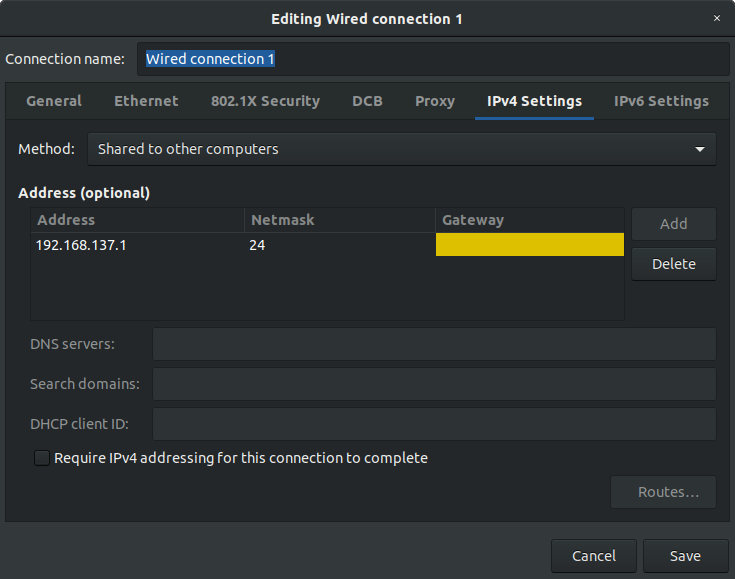
\includegraphics[width=0.6\columnwidth]{Figures/nm-connection-editor}
\caption{nm-connection-editor in Ubuntu 18.10}
\label{fig:nm-connection-editor}
\end{figure}


\subsubsection{Connecting to Eduroam - Raspbian Buster (Raspbian Site)}
These instructions come from \href{https://www.raspberrypi.org/forums/viewtopic.php?p=1501822#p1501822}{here}.\\

Unfortunately, when you use bleeding edge technology, you may end up cutting yourself. 
Raspbian Buster updates \verb|wpa_supplicant| to a version that doesn't have support for the authentication method used by Eduroam. So we need to roll back \verb|wpa_supplicant| to an older version. Ensure your Pi has internet access through a method such as Ethernet passthrough, and run the following:
\begin{lstlisting}
$ sudo apt-get remove wpasupplicant
\end{lstlisting}
Edit  /etc/apt/sources.list :
\begin{lstlisting}
$ sudo nano /etc/apt/sources.list
\end{lstlisting}
And change 
\begin{lstlisting}
deb http://raspbian.raspberrypi.org/raspbian/ buster main contrib non-free rpi
\end{lstlisting}
to 
\begin{lstlisting}
deb http://raspbian.raspberrypi.org/raspbian/ stretch main contrib non-free rpi
\end{lstlisting}
Run 
\begin{lstlisting}
$ sudo apt-get update
$ sudo apt-get install wpasupplicant
\end{lstlisting}
This will install the correct version of \verb|wpa_supplicant|. Check that \textbf{version 2.4} is installed by running
\begin{lstlisting}
$ wpa_supplicant -v
\end{lstlisting}
Now, change the sources file back.
\begin{lstlisting}
$ sudo nano /etc/apt/sources.list
\end{lstlisting}
And edit the contents to contain 
\begin{lstlisting}
deb http://raspbian.raspberrypi.org/raspbian/ buster main contrib non-free rpi
\end{lstlisting}
Finally, run 
\begin{lstlisting}
$ sudo apt-get update
\end{lstlisting}
To update sources
The correct version of \verb|wpa_supplicant| should now be installed, and you can configure your Pi for WiFi as you would if you were using Raspbian Stretch as explained in below.


\subsubsection{Connecting to Eduroam - Raspbian Stretch (Vula)}
This section provides the instructions on how to configure the Pi to use Eduroam. It is possible to do using the GUI through VNC, but we will not cover that here.

\begin{enumerate}
    \item SSH into your Pi.
    \item Generate a hash for your password. Take note of it as it is needed in a later step
    \begin{lstlisting}[gobble=4]
    $ echo -n your_uct_password_here | iconv -t utf16le | openssl md4
    \end{lstlisting}
    \item Open /etc/wpa\_supplicant/wpa\_supplicant.conf
    \begin{lstlisting}[gobble=4]
    $ sudo nano /etc/wpa_supplicant/wpa_supplicant.conf
    \end{lstlisting}
    \item Edit it so it looks as follows:
    \begin{lstlisting}[gobble=4]
    ctrl_interface=DIR=/var/run/wpa_supplicant GROUP=netdev
    update_config=1
    country=ZA

    network={
    ssid="eduroam"
    key_mgmt=WPA-EAP
    identity="studentnumber@wf.uct.ac.za"
    password=hash:generated_hash_from_earlier
    }
    \end{lstlisting}
    \item Save the file 
    \item Open \verb|/etc/dhcpcd.conf|
    \begin{lstlisting}[gobble=4]
    $ sudo nano /etc/dhcpcd.conf
    \end{lstlisting}
    \item Make sure the following lines are in the document:
    \begin{lstlisting}[gobble=4]
    interface wlan0
    metric 200
    \end{lstlisting}
    \item Reboot your Pi
    \item WiFi Generally takes a little longer to initialize than Ethernet, so give it time. You can see if it's ready by running 
    \begin{lstlisting}[gobble=4]
    $ ifconfig
    \end{lstlisting}
    And seeing if an IPv4 address ("inet") has been given.
    \item Test your configuration by pinging from the WiFi interface:
    \begin{lstlisting}[gobble=4]
    $ ping google.com -I wlan0
    \end{lstlisting}
\end{enumerate}

\subsection{Debugging Connections}
This section is a work in progress. As more common issues are reported by students, this section will be expanded.

\subsubsection{Note for Windows Users}
If you are having trouble accessing the internet from your Pi using the Ethernet Passthrough technique, it's likely the Windows bridge needs a reset. Change the IPv4 address of your Ethernet port to "Obtain an IP address automatically", then on your WiFi connection, disable sharing, click okay, and then re-enable sharing. Go back to the IP configuration of your Ethernet post, and double check the IP to see if it's been assigned 192.168.137.1. If not, you will need to change it using the "Advanced settings" button.

\subsubsection{WiFi}
See if you can see wireless networks.
\begin{lstlisting}
$ iwlist wlan0 scan
\end{lstlisting}

If you cannot connect via WiFi, enter into a shell on the Pi and run:
\begin{lstlisting}
$ journalctl -u wpa_supplicant | grep wlan0
$ journalctl -u dhcpcd.service | grep wlan0
\end{lstlisting}
This will output the log files and notify you of any incorrect configurations in wpa\_supplicant.

The following command will force the interface to be up (if it can be):
\begin{lstlisting}
sudo ifconfig wlan0 up
\end{lstlisting}

If all else fails, reboot and try again. Some services can be restarted without restarting the Pi, for example:
\begin{lstlisting}
sudo systemctl restart dhcpcd
\end{lstlisting}

\subsubsection{"Failure resolving URLs or "unknown host"}
If you try to ping a website and it fails, but pinging a URL works as expected, it is likely an issue with DNS configuration. Open the resolv.conf file:
\begin{lstlisting}
$ sudo nano /etc/resolv.conf
\end{lstlisting}
And edit it to read the following:
\begin{lstlisting}
nameserver 8.8.8.8
nameserver 192.168.137.1
\end{lstlisting}

8.8.8.8 is the IP of Google's DNS server. A DNS (Domain Name Service) server is responsible for converting human-readable addressed (for example google.co.za) to something the network architecture can understand (172.217.170.67, in this example).

If you still get this error, try running the following command:
\begin{lstlisting}
$ sudo route add default gw 192.168.137.1
\end{lstlisting}
Where the IP supplied is the IP of the computer or router you are connected to.

\subsection{Configuring the Pi to Act as an Access Point}
If you are hosting a server on the Raspberry Pi, or perhaps want to create a WiFi network for guests to connect to, the Pi can act as an access point. This guide comes from \href{https://www.raspberrypi.org/documentation/configuration/wireless/access-point.md}{https://www.raspberrypi.org/documentation/configuration/wireless/access-point.md} and \href{https://frillip.com/using-your-raspberry-pi-3-as-a-wifi-access-point-with-hostapd/}{https://frillip.com/using-your-raspberry-pi-3-as-a-wifi-access-point-with-hostapd/}. 

Note that this WiFi connection will not provide internet access by bridging the Ethernet port (that's something else entirely), but it works well for hosting services on the Pi, such as a Node-Red server.

\begin{enumerate}
\item SSH into the Pi, update, and reboot to ensure updates have taken place
\begin{lstlisting}
$ sudo apt-get update
$ sudo apt-get dist-upgrade
$ sudo reboot
\end{lstlisting}
\item Wait for the Pi to reboot, and reconnect via SSH. Install hostapd and dnsmasq
\begin{lstlisting}
$ sudo apt-get install hostapd dnsmasq
\end{lstlisting}
\item Configure a static IP in dhcpcd
\begin{lstlisting}
$ sudo nano /etc/dhcpcd.conf
\end{lstlisting}
Adjust the contents so that the wireless interface is described as follows:
\begin{lstlisting}    
interface wlan0
static ip_address=192.168.4.1/24
nohook wpa_supplicant
\end{lstlisting}
Save and close that file, and restart the dhcp service
\begin{lstlisting}
$ sudo systemctl restart dhcpcd
\end{lstlisting}
\item Run the following commands to create save the original dnsmasq, and create a new file which will be edited:
\begin{lstlisting}
$ sudo mv /etc/dnsmasq.conf /etc/dnsmasq.conf.orig
$ sudo nano /etc/dnsmasq.conf
\end{lstlisting}
Place the following in the now open file:
\begin{lstlisting}
interface=wlan0
listen-address=192.168.4.1
dhcp-range=192.168.4.2,192.168.4.180,255.255.255.0,24h
server=8.8.8.8
domain-needed
bogus-priv
\end{lstlisting}
Save and close the file
\item Restart the dnsmasq service
\begin{lstlisting}
$ sudo systemctl reload dnsmasq
\end{lstlisting}
% Configuring the access point host software (hostapd)
\item Configure hostapd. Open up the configuration file:
\begin{lstlisting}
sudo nano /etc/hostapd/hostapd.conf
\end{lstlisting}
Place the following configuration in the file. Some assumptions are made about the technical aspects of it, but these are beyond the scope of this course. Note that network name and password \textbf{do not} have quotes around them.
\begin{lstlisting}
interface=wlan0
driver=nl80211
ssid=TestNetwork
hw_mode=g
channel=7
ieee80211n=1
wmm_enabled=1
macaddr_acl=0
auth_algs=1
ignore_broadcast_ssid=0
wpa=2
wpa_passphrase=TestNetwork
wpa_key_mgmt=WPA-PSK
wpa_pairwise=TKIP
rsn_pairwise=CCMP
\end{lstlisting}
Save and close the file
\item Next, the system needs to know where to find this configuration file. Open the configuration file:
\begin{lstlisting}
$ sudo nano /etc/default/hostapd
\end{lstlisting}
Find the line with "\#DAEMON\_CONF" and replace it with:
\begin{lstlisting}
DAEMON_CONF="/etc/hostapd/hostapd.conf"
\end{lstlisting}
Save and close this file.
%  Start up
\item Now enable and start hostapd:
\begin{lstlisting}
$ sudo systemctl unmask hostapd
$ sudo systemctl enable hostapd
$ sudo systemctl start hostapd
\end{lstlisting}
\item Add routing and masquerade by opening sysctl:
\begin{lstlisting}
$ sudo nano /etc/sysctl.conf
\end{lstlisting}
And uncomment this line by removing the preceding \# symbol:
\begin{lstlisting}
net.ipv4.ip_forward=1
\end{lstlisting}
Save and close the file
\item Add a masquerade, and save the iptables rule:
\begin{lstlisting}
$ sudo iptables -t nat -A  POSTROUTING -o eth0 -j MASQUERADE
$ sudo sh -c "iptables-save > /etc/iptables.ipv4.nat"
\end{lstlisting}
\item Edit /etc/rc.local and add this just above "exit 0" to install these rules on boot.
\begin{lstlisting}
$ sudo nano /etc/rc.local
\end{lstlisting}
Place the following just above "exit 0" to install these rules on boot
\begin{lstlisting}
iptables-restore < /etc/iptables.ipv4.nat
\end{lstlisting}
\end{enumerate}

%% UART
\subsection{TTL over USB}

\textbf{Note:} The Pi uses 3.3V logic levels. Using a 5V logic module will permanently damage the pins.

This option allows you to use a USB to UART converter such as a FT232R or CP2102.
Begin by removing the SD card, and insert it into a computer. Make the following changes on the boot partition:

cmdline.txt: add the following (on the same line)
\begin{lstlisting}
console=serial0,115200 
\end{lstlisting}

config.txt
\begin{lstlisting}
uart_enable=1
dtoverlay=pi3-disable-bt
\end{lstlisting}
